\documentclass[9pt]{beamer}
% \documentclass[9pt]{article}
% \usepackage[noxcolor]{beamerarticle}
\usepackage[utf8]{inputenc}
\usepackage{CJKutf8} %japanese
\usepackage{tikz, tikz-cd}
\usepackage{hyperref}
\usepackage{graphicx}
\usepackage{ragged2e}
\usepackage{amsmath, amssymb}
\usepackage{wrapfig}
\usepackage{pifont}

\usetheme{Warsaw}
\usecolortheme{default}
\usefonttheme{structuresmallcapsserif}


%definitions
%============================================================
\title[Shinichi Mochizuki \hspace{25mm} \insertframenumber/\inserttotalframenumber]{
    Shinichi Mochizukithe\\ --the Japanese mathematician}
\subtitle{
    \textit{Mathematical proof that rocked number theory}}
    
\author{M.~Gruszczyński\inst{1} \and B.~Nems\inst{1}}
    \institute[WMiI]{
        \inst{1}%
        Faculty of Mathematics and Computer Science\\Uniwersity of Lodz}
        
\date[2020/2021]{
    
\includegraphics[width=2.25cm,height=0.75cm]{images/wmii.jpg}\\
    \textit{"Edycja tekstów naukowych", June 2021}}
    

% \logo{
%     \includegraphics[height=1cm]{overleaf-logo}}
\logo{
\begin{tikzpicture}
        \filldraw[fill=red!40](0,0) circle (0.30);
        \node[color=white](0,0) {\normalsize\textbf{UŁ}};
    \end{tikzpicture}}

\AtBeginSection{
    \begin{frame}
        \frametitle{Table of Contents}\tableofcontents[currentsection]
    \end{frame}
}

%presentation
%============================================================
\begin{document}
    \frame{\titlepage}

    \begin{frame}\label{init}
        \frametitle{Table of Contents}\tableofcontents
    \end{frame}
    
    \section{About Shinichi Mochizuki}
        
        %----------------------------------------------------
        \subsection{Shinichi Mochizuki}
        \begin{frame}
            \frametitle{Shinichi Mochizuki}
            
            \begin{center}
                \fbox{\begin{minipage}{33.5em}
                    \textbf{Shinichi Mochizuki (\begin{CJK}{UTF8}{min}望月 新一\end{CJK}, \textit{Mochizuki Shin'ichi}, born March 29, 1969)}
                \end{minipage}}
            \end{center}\vspace{0.1cm}
            
            \begin{columns}\label{mochizuki}
                \column{0.80\textwidth}
                    \justify
                    Mochizuki is a Japanese mathematician working in number theory and arithmetic geometry. He is one of the main contributors to anabelian geometry. His contributions include his solution of the Grothendieck conjecture in anabelian geometry about hyperbolic curves over number fields. Mochizuki has also worked in Hodge–Arakelov theory and p-adic Teichmüller theory. \\\vspace{0.50cm}
                    Mochizuki developed inter-universal Teichmüller theory, which has attracted a high level of attention of non-mathematicians due to claims it provides a resolution of the \hyperlink{abc}{\beamerbutton{abc conjecture}} (also known as Oesterl ́e–Masser conjecture).\\\vspace{0.50cm}
                    \only<article>{
                        Mochizuki entered Princeton University as an undergraduate at age 16 and graduated PhD salutatorian in 1988. After his PhD, Mochizuki spent two years at Harvard and then in 1994 moved back to Japan to join the Research Institute for Mathematical Sciences (RIMS) at Kyoto University in 1992, and was promoted to professor in 2002.
                    }
                \pause
                \column{0.15\textwidth}
                    \href{https://en.wikipedia.org/wiki/Shinichi_Mochizuki}{
                        
\includegraphics[width=1.25cm, height=1.25cm]{images/wiki.png}}
                    \vspace{0.8cm}
                    \href{https://www.kurims.kyoto-u.ac.jp/~motizuki/top-english.html}{
                        
\includegraphics[width=1.25cm, height=1.25cm]{images/home.png}}
            \end{columns}
        \end{frame}

        %----------------------------------------------------
        \subsection{ABC Conjecture}
        \begin{frame}\label{abc}
            \frametitle{ABC Conjecture}
            \begin{block}{Theory}
                For any real number $\epsilon > 0$, there exists a real number $K_{\epsilon} > 0$ such that
                $$c < K\epsilon \cdot \mathbf{rad}(abc)^{1+\epsilon}$$
                for any $abc$ triple $(a, b, c)$.
            \end{block}
            The conjecture says that $abc$ cannot have \textit{“too many”}repeated prime factors of \textit{“high multiplicity”} if $a + b = c,\text{ } gcd(a, b) = 1.$
            \pause
            \begin{example}
                For now the highest-quality triple (with a particularly small radical relative to $c$) is given below:\\\vspace{0.25cm}
                $a = 2$, $b = 3^{10} \cdot 109 = 6436341$, $c = 23^5 = 6436343$\\
                $\mathbf{rad}(abc) = 2\cdot 3\cdot 109\cdot 25 =15042$
            \end{example}
            \\\vspace{0.50cm}
            \only<article>{
                The abc conjecture expresses a profound link between the addition and multiplication of integer numbers. Any integer can be factored into prime numbers, its ‘divisors’: for example, 60 = 5 x 3 x 2 x 2. The conjecture roughly states that if a lot of small primes divide two numbers a and b, then only a few, large ones divide their sum, c.\\
                A proof, if confirmed, could change the face of number theory, by, for example, providing an innovative approach to proving Fermat’s last theorem, the legendary problem formulated by Pierre de Fermat in 1637 and solved only in 1994.
            }
        \end{frame}
        
        %----------------------------------------------------
        \subsection{Controversy}
        \begin{frame}
            \frametitle{Controversy}
                To quote \href{https://www.nature.com/articles/d41586-020-00998-2}{\textbf{\color{blue}NATURE}'s} 03 April 2020 article headline: \\
                \rotatebox{3}{
                    \emph{"Mathematical proof that rocked number theory will be published".}\\\vspace{0.25cm}}
            \begin{columns}
                \column{0.30\textwidth}
                    \vspace{0.5cm}
                    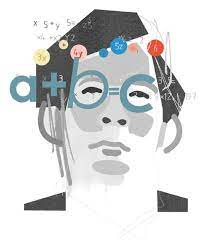
\includegraphics[width=3.5cm, height=4.75cm]{images/init.jpeg}
                \column{0.70\textwidth}
                    \justify
                    \textit{"After an eight-year struggle, embattled Japanese mathematician Shinichi Mochizuki has finally received some validation. His 600-page proof of the abc conjecture, one of the biggest open problems in number theory, has been accepted for publication.\\\vspace{0.35cm}
                    Acceptance of the work in Publications of the Research Institute for Mathematical Sciences (RIMS) is the latest development in a long and acrimonious controversy over the mathematician’s proof.\\\vspace{0.35cm}
                    (..) The paper “will have a big impact (..)"}
            \end{columns}
        \end{frame}
        
        %----------------------------------------------------
        \subsection{Proof chronology}
        \begin{frame}
            \frametitle{Proof chronology}
            \begin{center}
                \textbf{The controversy continues..}\\
            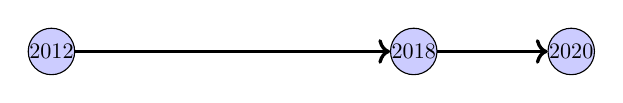
\begin{tikzpicture}[main node/.style={circle,fill=blue!20,draw,minimum size=0.4cm,inner sep=0pt,scale=0.8]}]
                \node[main node, left] at (0,0) (2012) {2012};
                \draw [very thick, ->] (2012) -- (4,0);
                \node[main node, right] at (4,0) (2018) {2018};
                \draw [very thick, ->] (2018) -- (6,0);
                \node[main node, right] at (6,0) (2020) {2020};
            \end{tikzpicture}
            \end{center}
            \begin{enumerate}[\ding{46}]
                \setbeamercovered{transparent}
                \setcounter{enumi}{0}
                \item<1-> 2012, Mochizuki posted four massive papers online, claiming to have solved the \textit{ABC Conjecture}.
                \begin{itemize}
                    \item Modest circumstances of publication of such an important work --'secret' announcement on the home page.
                    \item Written in an impenetrable, idiosyncratic style --"like you might be reading a paper from the future, or from outer space"
                \end{itemize}
                \item<1->  2018, Two highly respected mathematicians allegedly found a flaws in Mochizuki’s proof.
                \item<1> 2020, Acceptance of the work in Publications of the Research Institute for Mathematical Sciences (RIMS).
                \item<2-> \alert{However, the publication of the work by some seems to be unjustified.} --Edward Frenkel of the University of California, Berkeley, said: \textit{"I will withhold my judgement on the publication of this work until it actually happens, as new information might emerge."}          
            \end{enumerate}
        \end{frame}

    \section{About Japan country}
        
        %----------------------------------------------------
        \subsection{Japan}
        \begin{frame}
            \frametitle{Japan}
                \justify
                \fbox{
\includegraphics[width=.30cm,height=0.15cm]{images/flag.png}} \textbf{Japan} is the eleventh-most populous country in the world, as well as one of the most densely populated and urbanized. About three-fourths of the country's terrain is mountainous, concentrating its population of 125.36 million on narrow coastal plains. Japan is divided into 47 administrative prefectures and eight traditional regions. The Greater Tokyo Area is the most populous metropolitan area in the world, with more than 37.4 million residents.
                \begin{figure}[h]
                    \centering
                    
\includegraphics[width=0.7\textwidth]{images/japan.png}
                    \caption{Art depicting symbiosis of Japanese tradition and technology}
                    \label{fig:mesh1}
                \end{figure}
        \end{frame}

        %---------------------------------------------------------
        \subsection{Kyoto University}
        \begin{frame}
            \frametitle{Kyoto University}
            \begin{columns}
                \column{0.5\textwidth}
                    \begin{centering}
                        
\includegraphics[width=2cm,height=2cm]{images/uni.png}\\
                        \vspace{0.2cm}
                    \end{centering}
                    \justify
                    \textbf{Kyoto University} (\begin{CJK}{UTF8}{min}京都大学\end{CJK}, Kyōto daigaku), or KyotoU (\begin{CJK}{UTF8}{min}京大\end{CJK}, Kyōdai), is a public research university located in Kyoto, Japan. Founded in 1897, it is the second oldest university in Japan, one of the former Imperial Universities, the first three Designated National University and selected as a Top Type university of Top Global University Project by the Japanese government.
                \column{0.5\textwidth}
                    \justify
                    KyotoU is usually ranked amongst the top two in Japan, the top ten in Asia, and the world's top thirty institutions of higher education.\\\vspace{0.3cm}
                    \pause
                    \hyperlink{mochizuki}{\beamerbutton{Shinichi  Mochizuki}} spent two years at Harvard and then in 1994 moved back to Japan to join the Research Institute for Mathematical Sciences (RIMS) at Kyoto University in 1992, and was promoted to professor in 2002.\\\vspace{0.3cm}
                    \begin{centering}
                        % \begin{wrapfigure}{l}{0.35\textwidth}
                        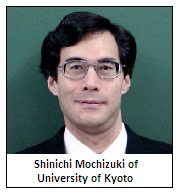
\includegraphics[width=1.8cm,height=2cm]{images/photo.jpg}\\
                        % \end{wrapfigure}
                    \end{centering}
                    \\\vspace{0.50cm}
                    \only<article>{
                        Kyoto University has generated 5 prime ministers of Japan to date, and is famed for producing world-class researchers. As of October 2019, 19 Nobel Prize laureates, 2 Fields medalists, and 1 Gauss Prize winner have been affiliated with Kyoto University, giving it the most Nobel laureates of all universities in Asia. Apart from distinguished politicians and scholars, the university also counts in its alumni esteemed medical and legal professionals, writers, artists, and business leaders.
                    }
            \end{columns}
        \end{frame}
        
    \section{The Bibliography}
    
        %---------------------------------------------------------
        \subsection{Picked sources}
        \begin{frame}
            \frametitle{Picked sources}
            \begin{thebibliography}{XXX}
                \bibitem[DC]{k1}D.Castelvecchi, \textit{Mathematical proof that rocked number theory will be published}, https://www.nature.com/articles/d41586-020-00998-2, 3 April 2020.
                \bibitem[ABC]{k1}ABC Conjecture, https://en.wikipedia.org/wiki/Abc\_conjecture, 28 May 2021.
                \bibitem[TU]{k1}Kyoto University, https://en.wikipedia.org/wiki/Kyoto\_University, 8 June 2021.
                \bibitem[JC]{k1}Japan, https://en.wikipedia.org/wiki/Japan, 8 June 2021.
                \bibitem[SM]{k1}Shinichi Mochizuki, https://en.wikipedia.org/wiki/Shinichi\_Mochizuki, 2 June 2021.
            \end{thebibliography}
        \end{frame}
        
        %---------------------------------------------------------
        \subsection{The End}
        \begin{frame}
            \frametitle{The End}
            \begin{center}
                Thanks for the attention!\\\vspace{0.25cm}
                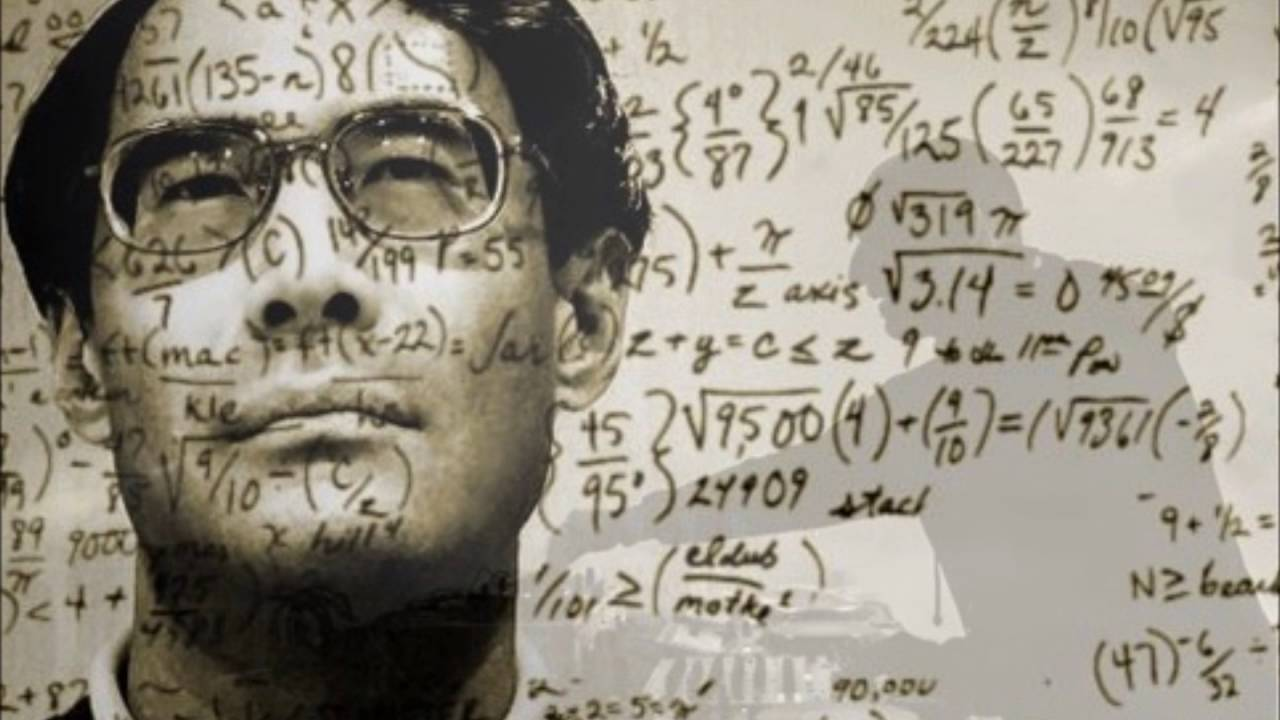
\includegraphics[width=8cm,height=4cm]{images/photo2.jpg}\\\vspace{0.25cm}
                \hyperlink{init}{\beamerbutton{start again \ding{220}}}\\
            \end{center}
        \end{frame}
    
\end{document}
